\documentclass[a4paper, 12pt, openany]{book}

%%% Работа с русским языком % для pdfLatex
\usepackage{cmap}					% поиск в~PDF
\usepackage{mathtext} 				% русские буквы в~фомулах
\usepackage[T2A]{fontenc}			% кодировка
\usepackage[utf8]{inputenc}			% кодировка исходного текста
\usepackage[english,russian]{babel}	% локализация и переносы
\usepackage{indentfirst} 			% отступ 1 абзаца
\usepackage{gensymb}				% мат символы?

%%% Работа с русским языком % для XeLatex
%\usepackage[english,russian]{babel}   %% загружает пакет многоязыковой вёрстки
%\usepackage{fontspec}      %% подготавливает загрузку шрифтов Open Type, True Type и др.
%\defaultfontfeatures{Ligatures={TeX},Renderer=Basic}  %% свойства шрифтов по умолчанию
%\setmainfont[Ligatures={TeX,Historic}]{Times New Roman} %% задаёт основной шрифт документа
%\setsansfont{Comic Sans MS}                    %% задаёт шрифт без засечек
%\setmonofont{Courier New}
%\usepackage{indentfirst}
%\frenchspacing

%%% Дополнительная работа с математикой
\usepackage{amsfonts,amssymb,amsthm,mathtools}
\usepackage{amsmath}
\usepackage{icomma} % "Умная" запятая: $0,2$ --- число, $0, 2$ --- перечисление
\usepackage{upgreek}

%% Номера формул
%\mathtoolsset{showonlyrefs=true} % Показывать номера только у тех формул, на которые есть \eqref{} в~тексте.

%%% Страница
\usepackage{extsizes} % Возможность сделать 14-й шрифт

%% Шрифты
\usepackage{euscript}	 % Шрифт Евклид
\usepackage{mathrsfs} % Красивый матшрифт

%% Свои команды
\DeclareMathOperator{\sgn}{\mathop{sgn}} % создание новой конанды \sgn (типо как \sin)
\DeclareMathOperator{\rg}{\mathop{rg}}
\DeclareMathOperator{\Rg}{\mathop{Rg}}
\DeclareMathOperator{\im}{\mathop{Im}}
\DeclareMathOperator{\tr}{\mathop{tr}}
\DeclareMathOperator{\const}{\mathop{const}}
\DeclareMathOperator{\Id}{\mathop{Id}}
%\DeclareMathOperator{\dim}{\mathop{dim}}
\usepackage{csquotes} % ещё одна штука для цитат
\newcommand{\pd}[2]{\ensuremath{\cfrac{\partial #1}{\partial #2}}} % частная производная
\newcommand{\abs}[1]{\ensuremath{\left|#1\right|}} % модуль
\renewcommand{\phi}{\ensuremath{\varphi}} % греческая фи
\newcommand{\pogk}[1]{\!\left(\cfrac{\sigma_{#1}}{#1}\right)^{\!\!\!2}\!} % для погрешностей


%\renewcommand{\labelenumi}{\asbuk{enumi})}

% Ссылки
\usepackage{color} % подключить пакет color
% выбрать цвета
\definecolor{BlueGreen}{RGB}{49,152,255}
\definecolor{Violet}{RGB}{120,80,120}
% назначить цвета при подключении hyperref
\usepackage[unicode, colorlinks, urlcolor=blue, linkcolor=blue, pagecolor=blue, citecolor=blue]{hyperref} %синие ссылки
%\usepackage[unicode, colorlinks, urlcolor=black, linkcolor=black, pagecolor=black, citecolor=black]{hyperref} % для печати (отключить верхний!)


%% Перенос знаков в~формулах (по Львовскому)
\newcommand*{\hm}[1]{#1\nobreak\discretionary{}
	{\hbox{$\mathsurround=0pt #1$}}{}}

%%% Работа с картинками
\usepackage{graphicx}  % Для вставки рисунков
\graphicspath{{images/}{images2/}}  % папки с картинками
\setlength\fboxsep{3pt} % Отступ рамки \fbox{} от рисунка
\setlength\fboxrule{1pt} % Толщина линий рамки \fbox{}
\usepackage{wrapfig} % Обтекание рисунков и таблиц текстом
\usepackage{multicol}

%%% Работа с таблицами
\usepackage{array,tabularx,tabulary,booktabs} % Дополнительная работа с таблицами
\usepackage{longtable}  % Длинные таблицы
\usepackage{multirow} % Слияние строк в~таблице
\usepackage{caption}
\captionsetup{labelsep=period, labelfont=bf}

%%% Оформление
\usepackage{indentfirst} % Красная строка
%\setlength{\parskip}{0.3cm} % отступы между абзацами
%%% Название разделов
\usepackage{titlesec}
\titlelabel{\thetitle.\quad}
\renewcommand{\figurename}{\textbf{Рис.}}		%Чтобы вместо figure под рисунками писал "рис"
\renewcommand{\tablename}{\textbf{Таблица}}		%Чтобы вместо table над таблицами писал Таблица
\usepackage{enumitem}
\setlist{nolistsep}
\usepackage{verbatim}

%%% Теоремы
\theoremstyle{plain} % Это стиль по умолчанию, его можно не переопределять.
\newtheorem{theorem}{Теорема}[section]
\newtheorem{proposition}[theorem]{Утверждение}
\newtheorem{predlog}{Предложение}[section]
\newtheorem{lemma}{Лемма}[section]

\theoremstyle{definition} % "Определение"
\newtheorem{definition}{Определение}[section]
\newtheorem{corollary}{Следствие}[theorem]
\newtheorem{problem}{Задача}[section]

\theoremstyle{remark} % "Примечание"
\newtheorem*{nonum}{Решение}
\newtheorem{zamech}{Замечание}[theorem]

%%% Правильные мат. символы для русского языка
\renewcommand{\epsilon}{\ensuremath{\varepsilon}}
\renewcommand{\phi}{\ensuremath{\varphi}}
\renewcommand{\kappa}{\ensuremath{\varkappa}}
\renewcommand{\le}{\ensuremath{\leqslant}}
\renewcommand{\leq}{\ensuremath{\leqslant}}
\renewcommand{\ge}{\ensuremath{\geqslant}}
\renewcommand{\geq}{\ensuremath{\geqslant}}
\renewcommand{\emptyset}{\varnothing}

%%% Для лекций по инфе
\usepackage{alltt}
\newcounter{infa}[section]
\newcounter{num}
\definecolor{infa}{rgb}{0, 0.2, 0.89}
\definecolor{infa1}{rgb}{0, 0.3, 1}
\definecolor{grey}{rgb}{0.5, 0.5, 0.5}
\newcommand{\tab}{\ \ \ }
\newcommand{\com}[1]{{\color{grey}\##1}}
\newcommand{\num}{\addtocounter{num}{1}\arabic{num}\tab}
\newcommand{\defi}{{\color{infa}def}}
\newcommand{\ini}{{\color{infa}in}}
\newcommand{\rangei}{{\color{infa}range}}
\newcommand{\fori}{{\color{infa}for}}
\newcommand{\ifi}{{\color{infa}if}}
\newcommand{\elsei}{{\color{infa}else}}
\newcommand{\printi}{{\color{infa1}print}}
\newcommand{\maxi}{{\color{infa}max}}
\newcommand{\classi}{{\color{infa}class}}
\newcommand{\returni}{{\color{infa}return}}
\newcommand{\elifi}{{\color{infa}elif}}


\newenvironment{infa}[1]{
	
	\vspace{0.5cm}
	\addtocounter{infa}{1}%
	\noindent{\large \textbf{Программа №\thesection.\arabic{infa}}}\textbf{<<#1>>}%
	\begin{alltt}%
	}{\end{alltt}
	\setcounter{num}{0}
	\vspace{0.1cm}}
%Пример кода:
%\begin{infa}{Поразрядная сортировка}
%	\ \num \defi count_sort(a):\tab \com{определяет нашу функцию}
%	\ \num \tab m = \maxi(a)+1
%	\ \num \tab q = [0]*m
%	\ \num \tab \fori x \ini a:
%	\ \num \tab \tab q[x] += 1
%	\ \num \tab pos = 0
%	\ \num \tab \fori x \ini q:
%	\ \num \tab \tab \fori i \ini \rangei(q[x]):
%	\ \num \tab \tab \tab a[pos] = x
%	\num \tab \tab \tab pos += 1
%\end{infa}

\usepackage{titlesec}
\titlelabel{\thetitle.\quad}

\usepackage{biblatex}
\addbibresource{references.bib}

\usepackage[left=1.27cm,right=1.27cm,top=2cm,bottom=2cm]{geometry}

\usepackage{fancyhdr} % Для колонтитулов

\renewcommand{\baselinestretch}{1.3}

\makeatletter % Убирает нумерацию на страницах, где \chapter
\renewcommand\chapter{\if@openright\cleardoublepage\else\clearpage\fi
	\thispagestyle{empty}% original style: plain
	\global\@topnum\z@
	\@afterindentfalse
	\secdef\@chapter\@schapter}
\makeatother

\usepackage{fancyhdr}
\pagestyle{fancy}
\fancyhf{}
\fancyhead[L]{\rightmark}
\fancyhead[R]{\textbf{\thepage}}

\setcounter{secnumdepth}{0}

\newcommand\invisiblesection[1]{%
	\refstepcounter{section}%
	\addcontentsline{toc}{section}{#1}%
	\sectionmark{#1}}


\title{Вопрос по выбору}
\author{Алексей Кожарин}
\date{\today}


\begin{document}
	
	\invisiblesection{Паулевский парамагнетизм электронов проводимости}
	\section{Парамагнитная восприимчивость электронов проводимости}
    Известно, что классическая теория свободных электронов не может дать удовлетворительного описания парамагнитной восприимчивости электронов проводимости в металле. 
    Каждый электрон обладает магнитным моментом, равным одному магнетону Бора $\mu_B$.
    Можно было бы ожидать, что электроны проводимости дадут в намагниченность металла парамагнитный вклад, описываемый \textbf{законом Кюри}:
    \begin{equation}
        \label{eq:curie_M}
        M=\frac{N \mu_{B}^{2}}{k_{B} T} B
    \end{equation}

    Напомним кратко, как он получается.
    Из-за наложения магнитного поля возникает небольшая анизотропия: какие-то направления спинов становятся выгодными, какие-то -- не очень.
    В приближении $\mu_B B \ll k_{B}T$ можно считать, что магнитный момент пропорционален отношению $\cfrac{\mu_{B}B}{k_{B}T}\, $ и задается формулой (\ref{eq:curie_M}).
    Тогда можно пересчитать магнитную восприимчивость по определению:
    \begin{equation*}
        \chi (T) = \cfrac{\partial M (T)}{\partial B}\, =
        \cfrac{N \mu_{B}^2}{k_{B}T}\, \propto \cfrac{1}{T}\,
        \Rightarrow \boxed{\chi (T) \propto \cfrac{1}{T}\, } .
    \end{equation*}

    Однако опыты показывают, что восприимчивость большинства нормальных неферромагнитных металлов не зависит от температуры,
    а величина ее может составлять лишь 1/100 от значения, предсказываемого формулой (\ref{eq:curie_M}) для комнатной температуры.

    \begin{wrapfigure}{l}{0.35\linewidth}
        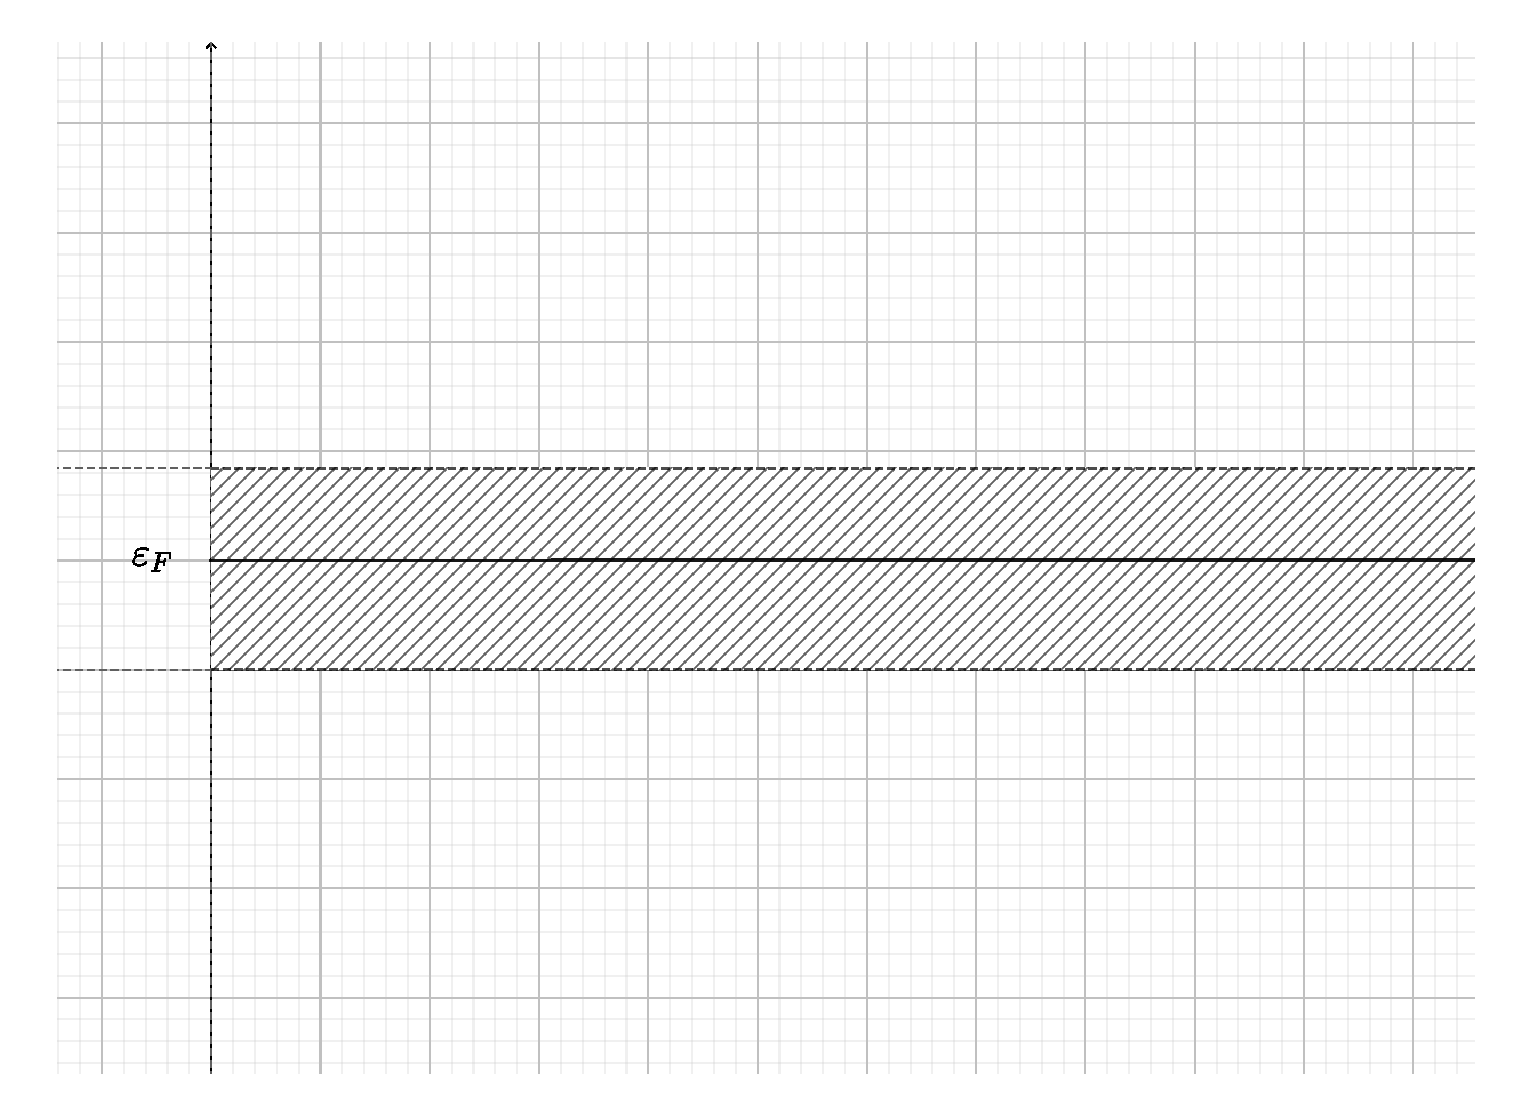
\includegraphics[width=\linewidth]{fermi_razm}
        \label{fig:fermi_razm}
        \caption{Размытие Ферми-поверхности при конечной температуре}
    \end{wrapfigure}

    Паули показал, что правильные результаты могут быть получены, если учесть, что электроны в металле подчиняются статистике Ферми-Дирака (\ref{eq:fermi_dirak_statistics}).
    Этой идее можно дать простое качественное объяснение.
    Для большинства электронов проводимости в металле вероятность того, что спиновый момент при включении внешнего поля повернется в направлении поля, равна нулю, поскольку состояния ниже уровня Ферми со спином вдоль поля в подавляющем числе уже заняты (в этом как раз есть учет статистики Ферми-Дирака).
    Только у небольшой части электронов с энергиями порядка $k_BT$, находящихся в верхней части фермиевского распределения, спины имеют шанс повернуться в направлении поля, и таким образом лишь доля $T/T_F$  от общего числа электронов дает вклад в восприимчивость.
    Это можно проиллюстрировать на рисунке слева.
    Следовательно,
    \begin{equation}
        M \approx \cfrac{N \mu^2 B}{k_{B}T}\, \cdot \cfrac{T}{T_F}\, = \cfrac{N \mu^2}{k_{B}T_{F}}\, B;
        \label{eq:M_pauli_approx}
    \end{equation}
    отсюда видно, что эта восприимчивость не зависит от температуры, а численная оценка полученного отношения дает значение наблюдаемого порядка величины.

    Вычислим теперь более строго выражение для парамагнитной восприимчивости свободного электронного газа при $T \ll T_{F}$ .
    При наложении магнитного поля спины электронов, сонаправленные с ним, примут меньшую энергию, а противонаправленные -- большую. Будем следовать методу расчета, наглядно иллюстрируемому схемой на рис. \ref{fig:parabola},~а).

    \begin{figure}[!h]
        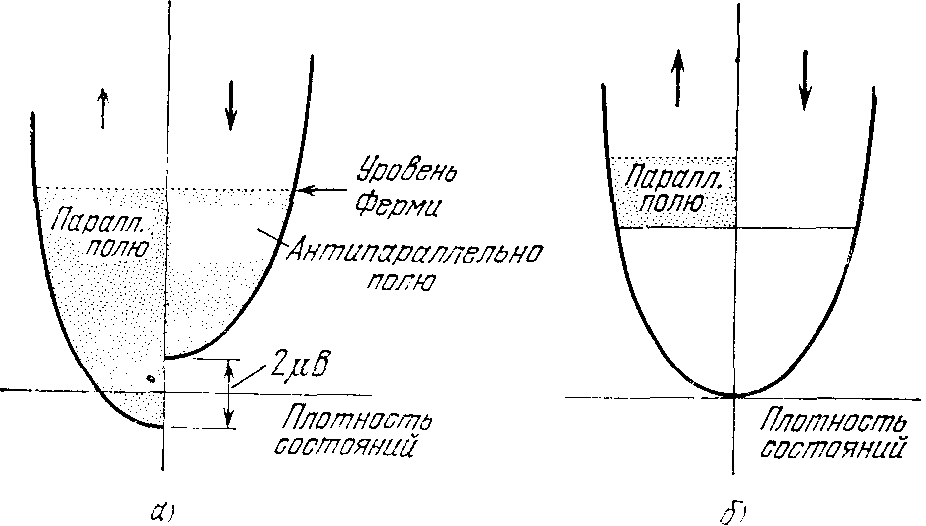
\includegraphics[width=\textwidth]{parabola}
        \caption{
        Электронный парамагнетизм Паули при $0^{\circ}$ K.
        Заштрихованная область на схеме а) описывает занятые уровни.
        Числа электронов в подзонах со спинами, направленными <<вверх>> (левая область) и <<вниз>> (правая область), определяются тем, что наивысший занятый уровень (для обеих областей) есть уровень Ферми.
        На схеме б) показан избыток спинов, направленных вверх, что вызвано действием внешнего магнитного поля.
    }
        \label{fig:parabola}
    \end{figure}
    Для концентрации электронов с магнитным моментом, параллельным магнитному полю, имеем:
    \begin{equation}
        N_{+}=\cfrac{1}{2} \int\limits_{-\mu B}^{\varepsilon_{F}} d \varepsilon f(\varepsilon) D(\varepsilon+\mu B) \approx \cfrac{1}{2} \int\limits_{0}^{\varepsilon_{F}} d \varepsilon f(\varepsilon) D(\varepsilon)+\cfrac{1}{2}\, \mu B D\left(\varepsilon_{F}\right)
        \label{eq:N+}
    \end{equation}
    где $f (\varepsilon)$ есть распределение Ферми-Дирака: 
    \begin{equation}
        f (\varepsilon) = \cfrac{1}{\exp\left(\varepsilon / (kT) \right) + 1}\, ,
        \label{eq:fermi_dirak_statistics}
    \end{equation}
    а $1 / 2 D(\varepsilon + \mu B)$ -- функция плотности состояний спинов одинаковой ориентации. Явное выражение для $D(\varepsilon)$ можно найти из его определения и предположения об изотропности:
    \begin{equation*}
        D(\varepsilon) = \cfrac{dN}{dE}\, = \left|
        \begin{array}{c}
            E = \cfrac{\hbar^2 k^2}{2m}\, ,
            ~ dE = \cfrac{\hbar^2k}{m}\, dk \\
            k = \sqrt{\cfrac{2m}{\hbar^2}\, E}, ~
            dk = \cfrac{m}{\hbar^2 k}\, dE \\
            dN = 2\cfrac{d^3k}{(2\pi)^3}\, = \cfrac{8 \pi k^2 dk}{8 \pi^3}\, = \cfrac{k^2 dk}{\pi^2}\, 
        \end{array}
        \right| = \cfrac{1}{2\pi^2}\, \left(\cfrac{2m}{\hbar^2}\, \right)^{3 / 2}  \sqrt{E} dE  
    \end{equation*}

    \begin{equation}
        D(\varepsilon_{F}) = 3N / 2\varepsilon_{F} = 
        3N / (2k_{B} T_{F})
        \label{eq:D_near_Fermi}
    \end{equation}

    Для спинов противоположной ориентации имеем сдвиг по энергиям на $\mu B$.

    В подсчете интеграла было два допущения.
    Во-первых, мы положили, что $k_{B}T \ll \varepsilon_{F}$.
    Во-вторых, ввиду малости энергии мы разложили $D(\varepsilon_{F})$ по Тейлору (откуда и вылезло $1 / 2$).

    Соответственно, для концентрации электронов с магнитным моментом, направление которого против поля $B$, имеем:
    \begin{equation}
        N_{-} = \cfrac{1}{2}\, \int\limits_{\mu B}^{\varepsilon_{F}} d\varepsilon f(\varepsilon) D(\varepsilon - \mu B) =
        \cfrac{1}{2}\, \int\limits_{0}^{\varepsilon_{F}} d\varepsilon f(\varepsilon) D(\varepsilon) - \cfrac{1}{2}\, \mu B D(\varepsilon_{F}).
        \label{eq:N-}
    \end{equation}
    Намагниченность, по определению, равна разности $N_{+} - N_{-}$, умноженной на магнитный момент~$\mu_{B}$~:
    \begin{equation}
        M = \mu_{B} (N_{+} - N_{-})
        \label{eq:M_definition}
    \end{equation}
    и, следовательно, получим:
    \begin{equation}
        \boxed{
            M \approx \mu_B^2 D(\varepsilon_{F}) B = 
            \cfrac{3 N\mu_B^2}{2k_{B} T_{F}}\, B,
        }
        \label{eq:M_pauli}
    \end{equation}
    где для $D(\varepsilon_F)$ использовано уже полученное выражение вблизи энергии Ферми (\ref{eq:D_near_Fermi}). Интегралы, которые мы не взяли, сократились.

    Результат (\ref{eq:M_pauli}) и есть формула для \textit{Паулевской спиновой намагниченности электрона проводимости}.

    При выводе этого соотношения предполагалось, что на пространственное перемещение электронов магнитное поле не влияет.
    Однако магнитное поле все-таки влияет на волновые функции электронов.
    Ландау показал, что для свободных электронов это обстоятельство приводит к возникновению диамагнитного момента, равного $-1 / 3$ от парамагнитного.
    Следовательно, полная намагниченность электронного газа равна:
    \begin{equation}
        M = \frac{3 N \mu^{2}}{2 k_{B} T_{F}} B - \frac{1}{3}\, \cdot  \frac{3 N \mu^{2}}{2 k_{B} T_{F}} B = 
        \cfrac{N \mu_{B}^2}{k_{B}T_{F}}\, B.
        \label{eq:M_with_landau_total}
    \end{equation}

    Чтобы сопоставить величину (\ref{eq:M_with_landau_total}) с наблюдаемыми значениями восприимчивости, следует еще учесть
    диамагнетизм ионных остовов,
    эффекты, связанные с энергетической зонной структурой
    и спин-спиновое взаимодействие.
    В металлическом натрии, к примеру, эффекты взаимодействия приводят к увеличению спиновой восприимчивости на 75\%.
    Однако рассмотрение этих эффектов весьма нетривиально. 

	
    \begin{thebibliography}{9}
        \bibitem{main}
        Ч. Киттель <<\textit{Введение в физику твердого тела}>>, с.534-538
    \end{thebibliography}
	
\end{document}
